\begin{tikzpicture}
\node[draw=white] (input) at (0,0){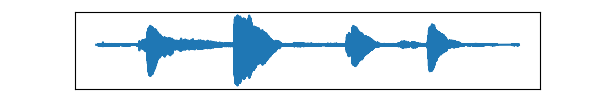
\includegraphics[width=0.62\textwidth]{./Chapter17/Figures/figure-hello-audio.png}};
\node[anchor=east,font=\scriptsize,align=center]  (a1) at  ([xshift=2.0em]input.west) {音频数据输入};
\node[minimum width=17.4em,minimum height=2.9em,draw=white,line width=3pt] at (0.3em,-0.02em){};

\node[anchor=north,draw,rounded corners=2pt,minimum width=16em, minimum height=2.2em,fill=yellow!20] (box) at ([xshift=0.4em]input.south){};
\node[anchor=west,minimum width=1.2em,minimum height=2.2em] (w1) at ([xshift=0.2em]box.west){{h}};
\node[anchor=west,minimum width=1.2em,minimum height=2.2em] (w2) at ([xshift=0.2em]w1.east){{e}};
\node[anchor=west,minimum width=1.2em,minimum height=2.2em] (w3) at ([xshift=0.2em]w2.east){{e}};
\node[anchor=west,minimum width=1.2em,minimum height=2.2em] (w4) at ([xshift=0.2em]w3.east){{$\epsilon$}};
\node[anchor=west,minimum width=1.2em,minimum height=2.2em] (w5) at ([xshift=0.2em]w4.east){{l}};
\node[anchor=west,minimum width=1.2em,minimum height=2.2em] (w6) at ([xshift=0.2em]w5.east){{$\epsilon$}};
\node[anchor=west,minimum width=1.2em,minimum height=2.2em] (w7) at ([xshift=0.2em]w6.east){{l}};
\node[anchor=west,minimum width=1.2em,minimum height=2.2em] (w8) at ([xshift=0.2em]w7.east){{l}};
\node[anchor=west,minimum width=1.2em,minimum height=2.2em] (w9) at ([xshift=0.2em]w8.east){{o}};
\node[anchor=west,minimum width=1.2em,minimum height=2.2em] (w10) at ([xshift=0.2em]w9.east){{o}};
\node[anchor=west,minimum width=1.2em,minimum height=2.2em] (w11) at ([xshift=0.2em]w10.east){{}};

\draw[very thick] (w1.south west) -- (w1.south east);
\draw[very thick] (w2.south west) -- (w2.south east);
\draw[very thick] (w3.south west) -- (w3.south east);
\draw[very thick] (w5.south west) -- (w5.south east);
\draw[very thick] (w7.south west) -- (w7.south east);
\draw[very thick] (w8.south west) -- (w8.south east);
\draw[very thick] (w9.south west) -- (w9.south east);
\draw[very thick] (w10.south west) -- (w10.south east);
%\draw[very thick] (w11.south west) -- (w11.south east);

\node[anchor=north,minimum width=1.2em,minimum height=1.4em,fill=gray!30] (m1) at ([yshift=-1em]w1.south){{h}};
\node[anchor=north,minimum width=2.64em,minimum height=1.4em,fill=gray!30] (m2) at ([yshift=-1em,xshift=0.72em]w2.south){{e}};
\node[anchor=north,minimum width=1.2em,minimum height=1.4em,fill=gray!30] (m3) at ([yshift=-1em]w4.south){};
\node[anchor=north,minimum width=1.2em,minimum height=1.4em,fill=gray!30] (m4) at ([yshift=-1em]w5.south){{l}};
\node[anchor=north,minimum width=1.2em,minimum height=1.4em,fill=gray!30] (m5) at ([yshift=-1em]w6.south){};
\node[anchor=north,minimum width=2.64em,minimum height=1.4em,fill=gray!30] (m6) at ([yshift=-1em,xshift=0.72em]w7.south){{l}};
\node[anchor=north,minimum width=2.64em,minimum height=1.4em,fill=gray!30] (m7) at ([yshift=-1em,xshift=0.72em]w9.south){{o}};
\node[anchor=north,minimum width=1.2em,minimum height=1.4em,fill=gray!30] (m8) at ([yshift=-1em]w11.south){};

\node[anchor=north,minimum width=1.2em,minimum height=1.4em,fill=gray!30] (o1) at ([yshift=-3.8em]w1.south){{h}};
\node[anchor=north,minimum width=1.2em,minimum height=1.4em,fill=gray!30] (o2) at ([yshift=-3.8em]w2.south){{e}};
\node[anchor=north,minimum width=1.2em,minimum height=1.4em,fill=gray!30] (o3) at ([yshift=-3.8em]w3.south){{l}};
\node[anchor=north,minimum width=1.2em,minimum height=1.4em,fill=gray!30] (o4) at ([yshift=-3.8em]w4.south){{l}};
\node[anchor=north,minimum width=1.2em,minimum height=1.4em,fill=gray!30] (o5) at ([yshift=-3.8em]w5.south){{o}};
\node[anchor=north,minimum width=1.2em,minimum height=1.4em,fill=gray!30] (o6) at ([yshift=-3.8em]w6.south){};
\node[anchor=north,minimum width=1.2em,minimum height=1.4em,fill=gray!30] at ([yshift=-3.8em]w7.south){};
\node[anchor=north,minimum width=1.2em,minimum height=1.4em,fill=gray!30] at ([yshift=-3.8em]w8.south){};
\node[anchor=north,minimum width=1.2em,minimum height=1.4em,fill=gray!30] at ([yshift=-3.8em]w9.south){};
\node[anchor=north,minimum width=1.2em,minimum height=1.4em,fill=gray!30] at ([yshift=-3.8em]w10.south){};
\node[anchor=north,minimum width=1.2em,minimum height=1.4em,fill=gray!30] at ([yshift=-3.8em]w11.south){};

\draw[blue!40,fill=blue!30,opacity=0.7] (w1.south west) -- (w1.south east) -- (o1.south east) -- (o1.south west) -- (w1.south west);
\draw[blue!40,fill=blue!30,opacity=0.7] (w2.south west) -- (w3.south east) -- (m2.south east) .. controls ([yshift=-0.3em]m2.south east) and ([yshift=0.3em]o2.north east) .. (o2.north east) -- (o2.south east) -- (o2.south west) -- (w2.south west);
\draw[blue!40,fill=blue!30,opacity=0.7] (w5.south west) -- (w5.south east) -- (m4.south east) .. controls ([yshift=-0.3em]m4.south east) and ([yshift=0.3em]o3.north east) .. (o3.north east) -- (o3.south east) -- (o3.south west) -- (o3.north west) .. controls ([yshift=0.3em]o3.north west) and ([yshift=-0.3em]m4.south west) .. (m4.south west) -- (w5.south west);
\draw[blue!40,fill=blue!30,opacity=0.7] (w7.south west) -- (w8.south east) -- (m6.south east) .. controls ([yshift=-0.3em]m6.south east) and ([yshift=0.3em]o4.north east) .. (o4.north east) -- (o4.south east) -- (o4.south west) -- (o4.north west) .. controls ([yshift=0.3em]o4.north west) and ([yshift=-0.3em]m6.south west) .. (m6.south west) -- (w7.south west);
\draw[blue!40,fill=blue!30,opacity=0.7] (w9.south west) -- (w10.south east) -- (m7.south east) .. controls ([yshift=-0.1em]m7.south east) and ([yshift=0.2em]o5.north east) .. (o5.north east) -- (o5.south east) -- (o5.south west) -- (o5.north west) .. controls ([yshift=0.1em]o5.north west) and ([yshift=-0.5em]m7.south west) .. (m7.south west) -- (w9.south west);
%\draw[blue!40,fill=blue!30,opacity=0.7] (w11.south west) -- (w11.south east) -- (m8.south east) .. controls ([yshift=-0.4em]m8.south east) and ([yshift=0.1em]o6.north east) .. (o6.north east) -- (o6.south east) -- (o6.south west) -- (o6.north west) .. controls ([yshift=0.1em]o6.north west) and ([yshift=-0.5em]m8.south west) .. (m8.south west) -- (w11.south west);

\node[anchor=north,font=\scriptsize,align=center] (a2) at  ([yshift=-1.4em]a1.south) {预测字母序列};
\node[anchor=north,font=\scriptsize,align=center] (a3) at  ([yshift=-1.8em]a2.south) {合并重复字母 \\ 并丢弃$\epsilon$};
\node[anchor=north,font=\scriptsize,align=center] (a4) at  ([yshift=-0.6em]a3.south) {最终结果输出};
\end{tikzpicture}